\section{Fitness Function}
The fitness function is the essential part of the GA that assesses the solutions. The target solution's fitness function value is the minimum or maximum of the fitness function, depending on the fitness function design. There are no general rules for its range of values and only simple recommendations for its creation. The target value of average maintained illuminance and the target value of uniformity are watched in the algorithm. The output design is the most effective and the cheapest after the target values are reached with minimum count of luminaires. Therefore the minimization of the luminaires count is also expected.

%TODO viz XXX
The first attempt to create a suitable fitness function was based on the idea, that the minimum luminaire number needed for the required target illuminance was XXX. The fitness function consisted of the sum of two parts $g_1$, $g_2$ defined as follows:

\begin{equation}
\label{eq:fitV1}
f\left(\overline{E}_{m}, U_0\right) = g_1\left(\overline{E}_{m}\right) + g_2\left(U_0\right)
\end{equation}

\begin{equation}
\label{eq:fitV1G1}
	g_1\left(\overline{E}_{m}\right)=
	\begin{cases} 
		e^{\frac{\overline{E}_{m}-\overline{E}_{mT}}{\overline{E}_{m}}} & \left( 0, \overline{E}_{mT}\right\rangle\\
		e^{\frac{\overline{E}_{mT}-\overline{E}_{m}}{\overline{E}_{m}}} & \left( \overline{E}_{mT}, \infty\right)
	\end{cases}
\end{equation}

\begin{equation}
\label{eq:fitV1G2}
	g_2\left(U_0\right)=
	\begin{cases} 
		\frac{U_0}{2\cdot U_{0T}} & \left\langle 0, U_{0T}\right\rangle\\
		1-\frac{e^{\frac{U_{0T}-U_0}{U_{0T}}}}{2} & \left( U_{0T}, \infty\right)
	\end{cases}
\end{equation}

\noindent where:
\begin{description}
	\item[$\overline{E}_{m}$] is the calculated maintained average value of illuminance,
	\item[$\overline{E}_{mT}$] is the target maintained average value of illuminance,
	\item[$U_0$] is the calculated lighting uniformity,
	\item[$U_{0T}$] is the target lighting uniformity.
\end{description}

Exponential functions were used for both parts. Each part could reach a maximum of $1$. Function~\ref{eq:fitV1G1} respected the requirements of the target illuminance. The maximum was reached exactly for the target illuminance value. As seen in Figure~\ref{fig:fitV1G1G2}, according to the definition functional values greater than the maximum were preferred to smaller values due to a slower decrease of the functional value for this part of the interval. The limits at both bounds of the definition interval reached zeros:

\begin{equation}
\label{eq:g1lim0}
\lim_{\overline{E}_{m}\to 0+} g_1\left(\overline{E}_{m}\right) = 0
\end{equation}
\begin{equation}
\label{eq:g1limInf}
\lim_{\overline{E}_{m}\to \infty} g_1\left(\overline{E}_{m}\right) = e^{-1}
\end{equation}

Function~\ref{eq:fitV1G1} respected the requirements for uniformity and it was linear until it reached the target value. Then the exponential function created the saturation effect.

According to the designed fitness function, the algorithm was supposed to reach the target value of illuminance with the highest possible uniformity. However only the restriction of getting the exact value of the illuminance was not sufficient to get the minimum count of luminaires. The demand to maximize uniformity favored solutions with little bit more luminaires than needed to fulfill the minimum illuminance requirement. Although this fact could be fixed by adding a weight multiplier either to Equation~\ref{eq:fitV1G1} or \ref{eq:fitV1G2}, the function did not seem to be further suitable for the algorithm and optimization. Mainly because it could hardly include any designer's preferences and the calculations of exponential functions were time consuming.

\begin{figure}[htb]
  \centering
  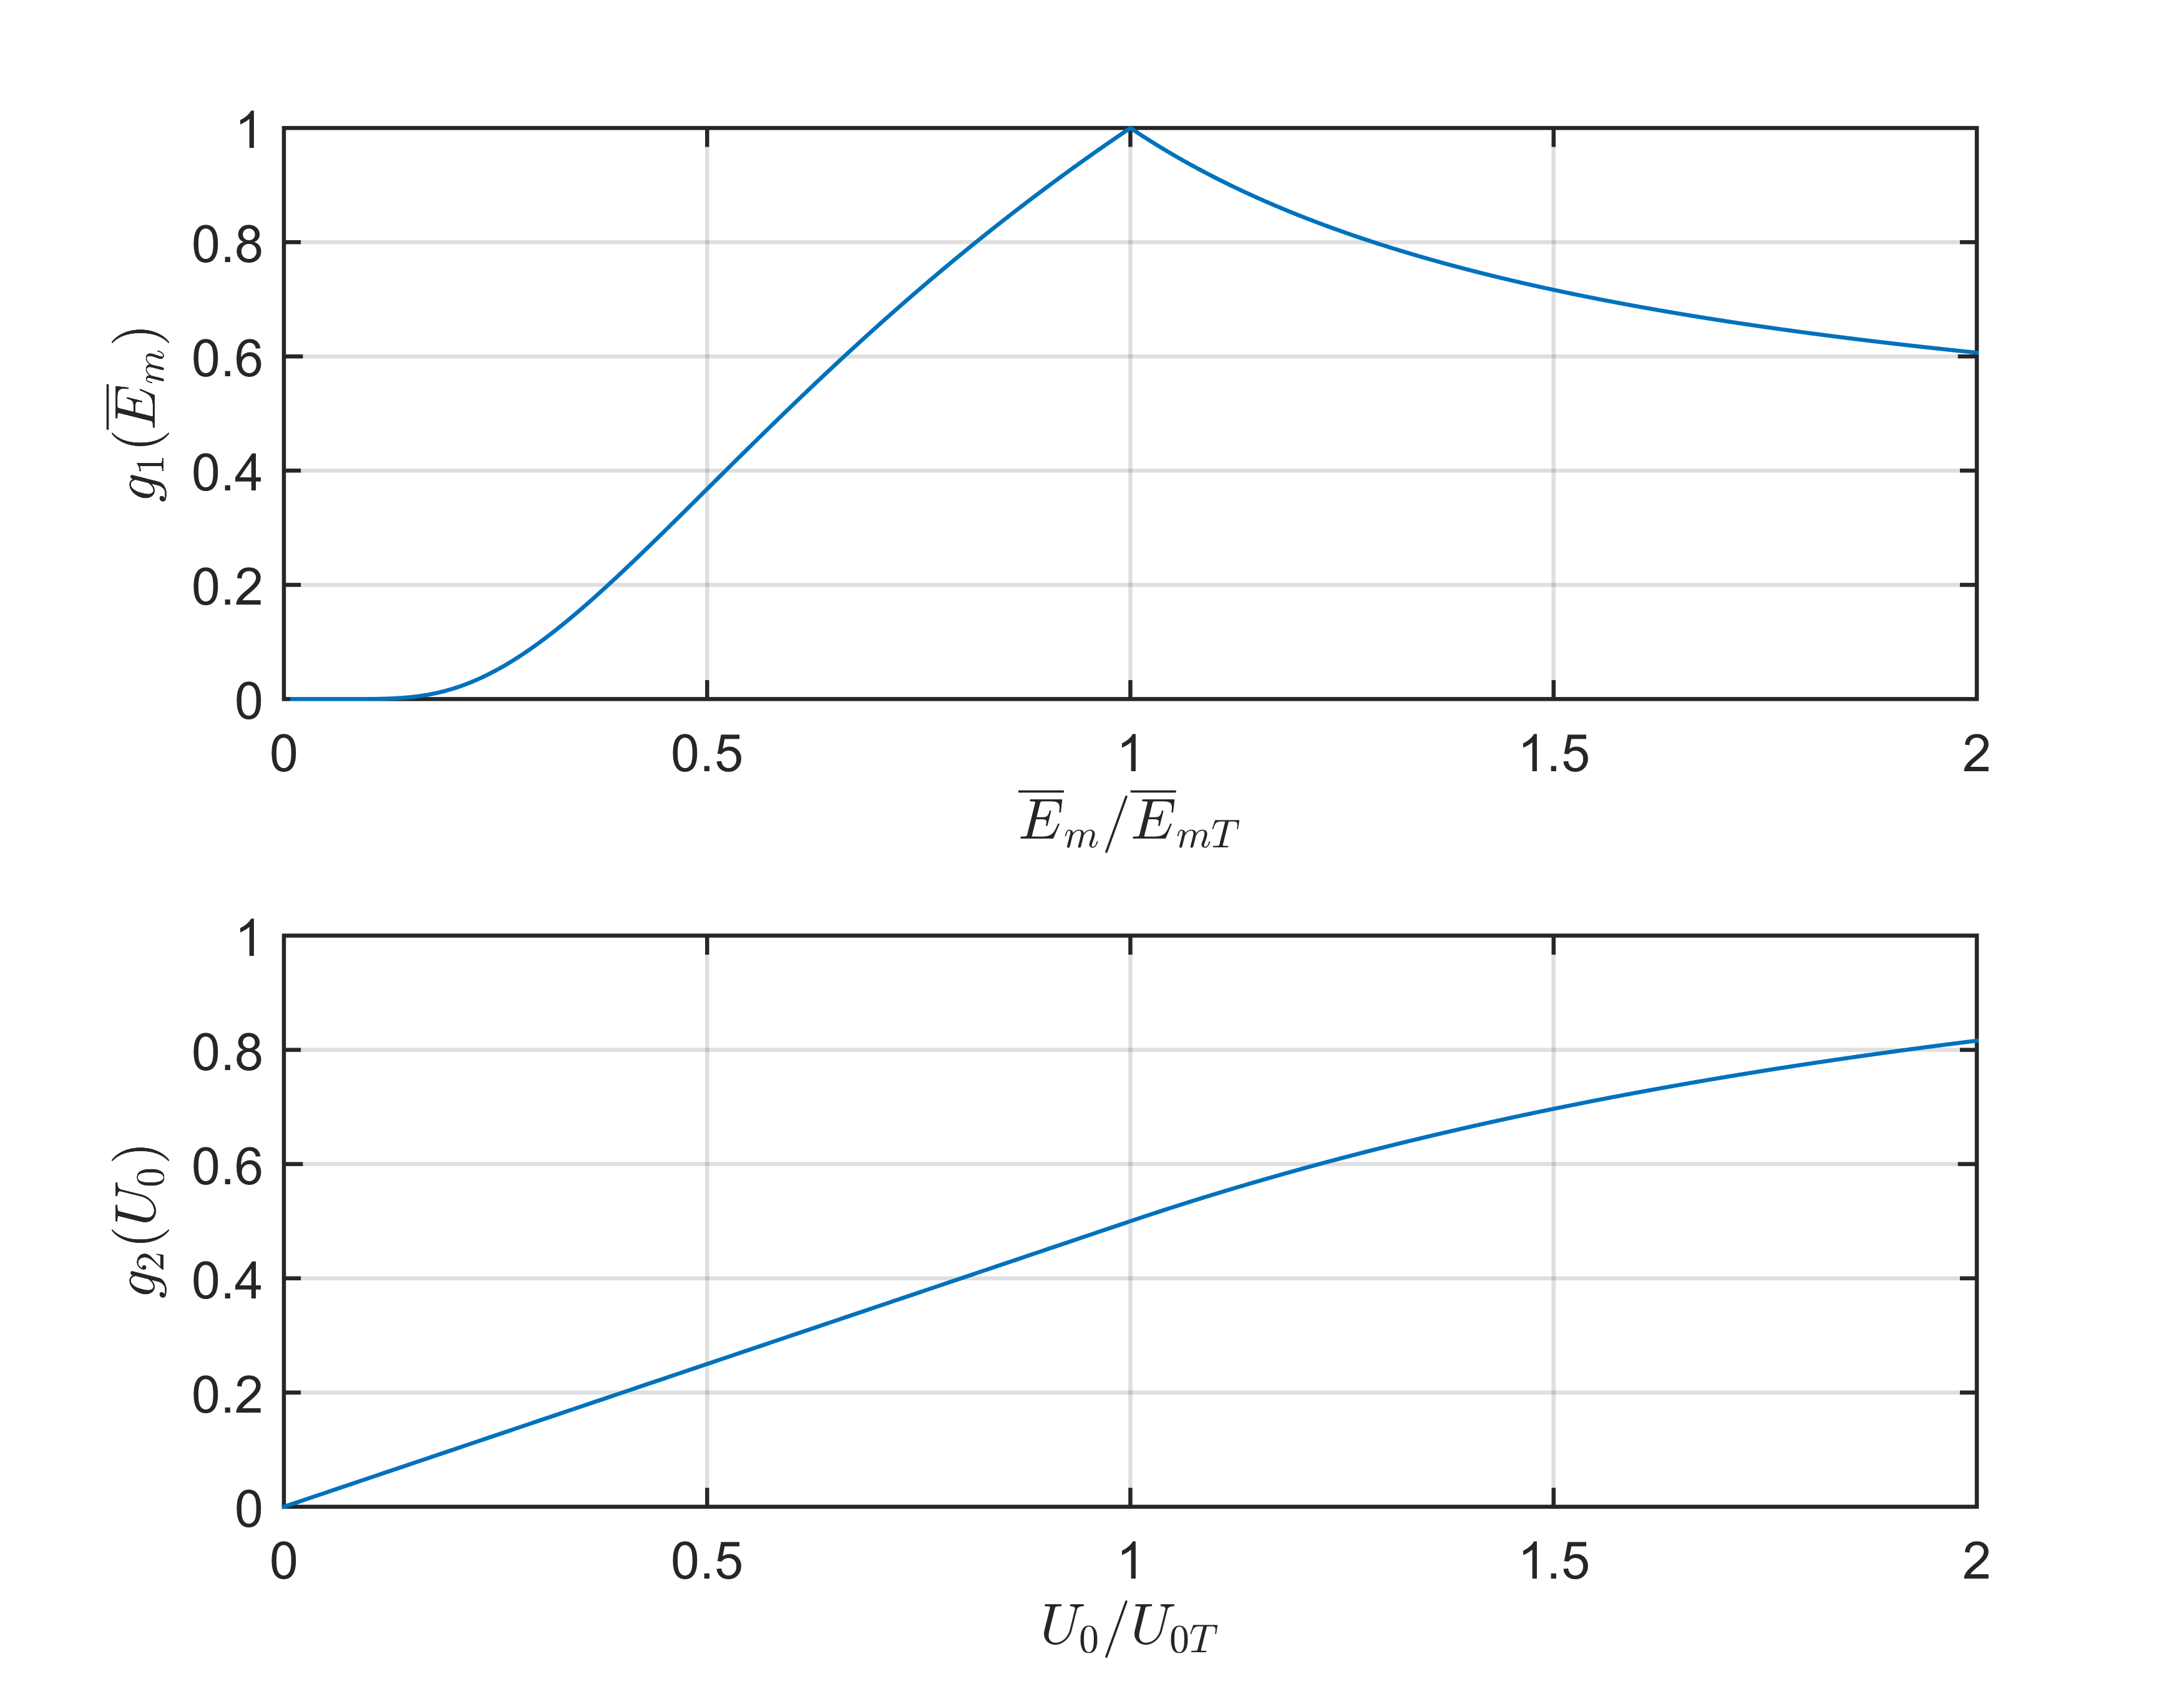
\includegraphics[width=\columnwidth]{obrG1G2}
  \caption{Graphs of parts $g_1\left(\overline{E}_{m}\right)$ and $g_2\left(U_0\right)$ of the fitness function}
  \label{fig:fitV1G1G2}
\end{figure}

The fitness function bellow is currently used in the algorithm. Solutions that do not reach basic requirements of target illuminance or uniformity are evaluated by length of the chromosome $L$:

\begin{equation}
\label{eq:fitV2EUA}
	f\left(C,\overline{E}_{m}, U_0\right)= L
\end{equation}

\noindent Otherwise the fitness is evaluated by:

\begin{equation}
\label{eq:fitV2EUB}
\begin{split}
f\left(C, \overline{E}_{m}, U_0\right)&=C +\\
& + \left( 1 - \alpha\right)\cdot\frac{\overline{E}_{mT}}{\overline{E}_{m}+\epsilon} + \\
& + \alpha\cdot\frac{U_{0T}}{U_0 + \epsilon}
\end{split}
\end{equation}

\noindent where:
\begin{description}
	\item[$C$] is the count of luminaires,
	\item[$\overline{E}_{m}$] is the calculated maintained average value of illuminance,
	\item[$\overline{E}_{mT}$] is the target maintained average value of illuminance,
	\item[$U_0$] is the calculated lighting uniformity,
	\item[$U_{0T}$] is the target lighting uniformity,
	\item[$\alpha$] is a number between 0 and 1,
	\item[$\epsilon$] is a very small number, that prevents the division by 0.
\end{description}

$\alpha$ represents the designer's intention to prefer one of the parameter to another. The target ratio between relative values of the parameters can be obtained from partial derivation of the fitness function:

\begin{equation}
\label{eq:fitV2ratio}
R =\frac{\overline{E}_{m}}{\overline{E}_{mT}}\cdot\frac{U_{0T}}{U_0}=\sqrt{\frac{1-\alpha}{\alpha}}
\end{equation}

\noindent There is no preference if $\alpha$ is equal to $0.5$.

This fitness function is supposed to be minimized. Equation \ref{eq:fitV2EUB} can be, if close to the target values of illuminance and uniformity, separated into an integer part, given only by the count of luminaires $h_1\left(C\right)= C$ and a fraction part that is given by:

\begin{equation}
\label{eq:fitV2frac}
	h_2\left(\overline{E}_{m}, U_0\right)= \left( 1 - \alpha\right)\cdot\frac{\overline{E}_{mT}}{\overline{E}_{m}+\epsilon} + \alpha\cdot\frac{U_{0T}}{U_0 + \epsilon}
\end{equation}

The main impact of the integer part $h_1\left(C\right)$ occurs at the beginning of the optimization. Only solutions that fulfill the standard requirements can have a smaller value of fitness than the length of its chromosome. For other solutions the most effective way to minimize the outcome of Equation~\ref{eq:fitV2EUB} is by decreasing the count of luminaires. Changes of part $h_2\left(\overline{E}_{m}, U_0\right)$ are less significant, because for high counts of luminaires, the denominator of Equation~\ref{eq:fitV2frac} is much higher than the numerator. Therefore the resulting fraction is very small.

After getting the optimal count of luminaires, function's $h_2\left(\overline{E}_{m}, U_0\right)$ output value will be close to 1 but smaller. An effective way to minimize Equation~\ref{eq:fitV2EUB} is to get the highest possible illuminance and uniformity for the given number of luminaires.

The defined fitness function was used for several runs of the GA and has always worked well. However there is a known problem in the definition of Equation~\ref{eq:fitV2EUA}. Consider the case, that none of the initial solutions would fulfill the standard requirements. Then all of them would have the same  fitness value equal to length of the chromosome $L$. It is very probable, that after selection, crossovers and mutations at least a single solution will appear fulfilling the standard requirements. But there can also be rare cases, in which the algorithm never optimizes the count of luminaires, because the fitness function in these cases is independent on all parameters of solutions. The presence of the problem is more probable for very small population sizes, small count of generations, small probability of mutations or for an inappropriately designed selection method.

Some parameter dependency ca be added to Equation~\ref{eq:fitV2EUA}. However it was quite useless for the further described settings of the GA and the chosen selection method. It would be extremely rare if any of the solutions fulfilling the standard requirements would not appear after a couple of generations.
